% -*- latex -*-
%%%%%%%%%%%%%%%%%%%%%%%%%%%%%%%%%%%%%%%%%%%%%%%%%%%%%%%%%%%%%%%%
%%%%
%%%% This TeX file is part of the course
%%%% Scientific Computing in C++23
%%%% copyright 2023-2024 Victor Eijkhout eijkhout@tacc.utexas.edu
%%%%
%%%% d2dtests.tex : test results
%%%%
%%%%%%%%%%%%%%%%%%%%%%%%%%%%%%%%%%%%%%%%%%%%%%%%%%%%%%%%%%%%%%%%

\Level 0 {Introduction}

In this paper we evaluate multiple parallel programming models
with respect to both ease of expression, and resulting performance.
We do this by implementing the mathematical algorithm
known as the `power method' in a variety of ways,
using modern C++ technniques.

\Level 0 {Algorithm aspects}

%% ALGORITHM DISCUSSION REMOVED TO SATSIFY SC PAGE LIMIT.
%% THIS CAN BE REINSTATED FOR FINAL SUBMISSION.

%% \begin{comment}
We briefly discuss the power method, mostly going into
its computational aspects.
For the mathematical side, see \HPSCref{app:power-method}.

%%packtsnippet d2dpower
Computationally, the power method is an attractive paradigmatic example
in that it exhibits the most common parallelism patterns:
\begin{itemize}
\item independent or `convenient' parallelism;
\item global reduction operations
\item point-to-point communications.
\end{itemize}
As follows.
The method is given by
\begin{quote}
  \begin{tabbing}
    Let $A$ a matrix of interest\\
    Let $x$ be a random vector\\
    For \=iterations until convergence\\
    \> compute the product $y\leftarrow Ax$\\
    \> compute the norm $\gamma=\| y \|$\\
    \> normalize $x\leftarrow y/\gamma$\\
  \end{tabbing}
\end{quote}
where in the limit $\gamma$ will be the
largest eigenvalue of~$A$,
and $x$ the corresponding eigenvector.

The basis to parallelizing the power method lies in the distribution of~$x$.
Each processing element~$p$, whether that be a core or processor,
takes care (in a sense that we will later defined)
of a disjoint set of indices~$I_p$.
The operations then are:
\begin{itemize}
\item The normalization step has independent parallelism:
  each component $y_i=x_i/\gamma$ can be independently computed,
  so each process~$p$ can compute $y_i$ for~$i\in I_p$ fully independently;
\item Computing $\gamma$ is a all-reduction:
  each processing element $p$ first computes $\gamma_p=\sqrt{\sum_{i\in I_p}y_i^2}$
  independently,
  and $\gamma=\sqrt{\sum_p\gamma_p}$ is then formed by combination, and
  made available to all~$p$;
\item Finally, for the operator $A$ we assume a sparse matrix,
  for instance a \acf{FD} stencil for a \ac{PDE}, or a \indexterm{convolution} kernel.
  This is characterized by each component $y_i$ of the output needing several
  components $x_j$ of the input. In our case, putting a two-dimensional
  indexing on the vectors:
  \[ y_{ij} = 4x_{ij} - x_{i-1,j} -x_{i+1,j} - x_{i,j-1} - x_{i,j+1} \]
\end{itemize}
%%packtsnippet end

%% \end{comment}

\Level 1 {Loop parallelism}
%%packtsnippet d2dloops
\label{sec:d2d-omp1d}

In our power method application
\begin{packt}
  (chapter~\ref{ch:parexample})
\end{packt}
a first example of a parallel loop is scaling an array by a factor.
%
\cxxverbatimsnippet{d2dscaleseq}
%
where \lstinline{m,n} are the size of the domain and \lstinline{b}~is the
width of a halo region.

Some remarks:
\begin{enumerate}
\item We use template parameters \lstinline{idxint} and \lstinline{real}
  for integers and floating point quantities, respectively.
\item
  The loops range only over the $m\times n$ interior part of the domain,
  which is allocated with size $(m+2b)\times(n+2b)$.
  %% of the \lstinline{mdspan}.
  %% Later we will explore using a range-based loop and
  %% dispensing with indexing entirely.
  %% However, that is not always possible.
\item We are using a traditional macro to translate from two-dimensional
  to one-dimensional indexing, skipping the border points:
  \cxxverbatimsnippet{d2dseqindex}
  Later we will discuss other indexing schemes.
\begin{packt}
    (For the macro idiom, see section~\ref{sec:cpp-mac-param}.)
\end{packt}
\item
  For the initial implementation, the \lstinline{out,in} data
  are \lstinline{double*} pointers, for instance obtained
  as the \lstinline{data} member of a \lstinline{std::vector}.
  Later we will explore implementing the data as an \lstinline{mdspan} object
  so we can use the two-dimensional \lstinline{[i,j]} type indexing.
\end{enumerate}
%%packtsnippet end

\Level 1 {Reduction}
%%packtsnippet d2dreduction

The $\ell_2$ reduction of our example application
looks in code like:
%
\cxxverbatimsnippet{d2dnormseq}

\begin{figure}[t]
  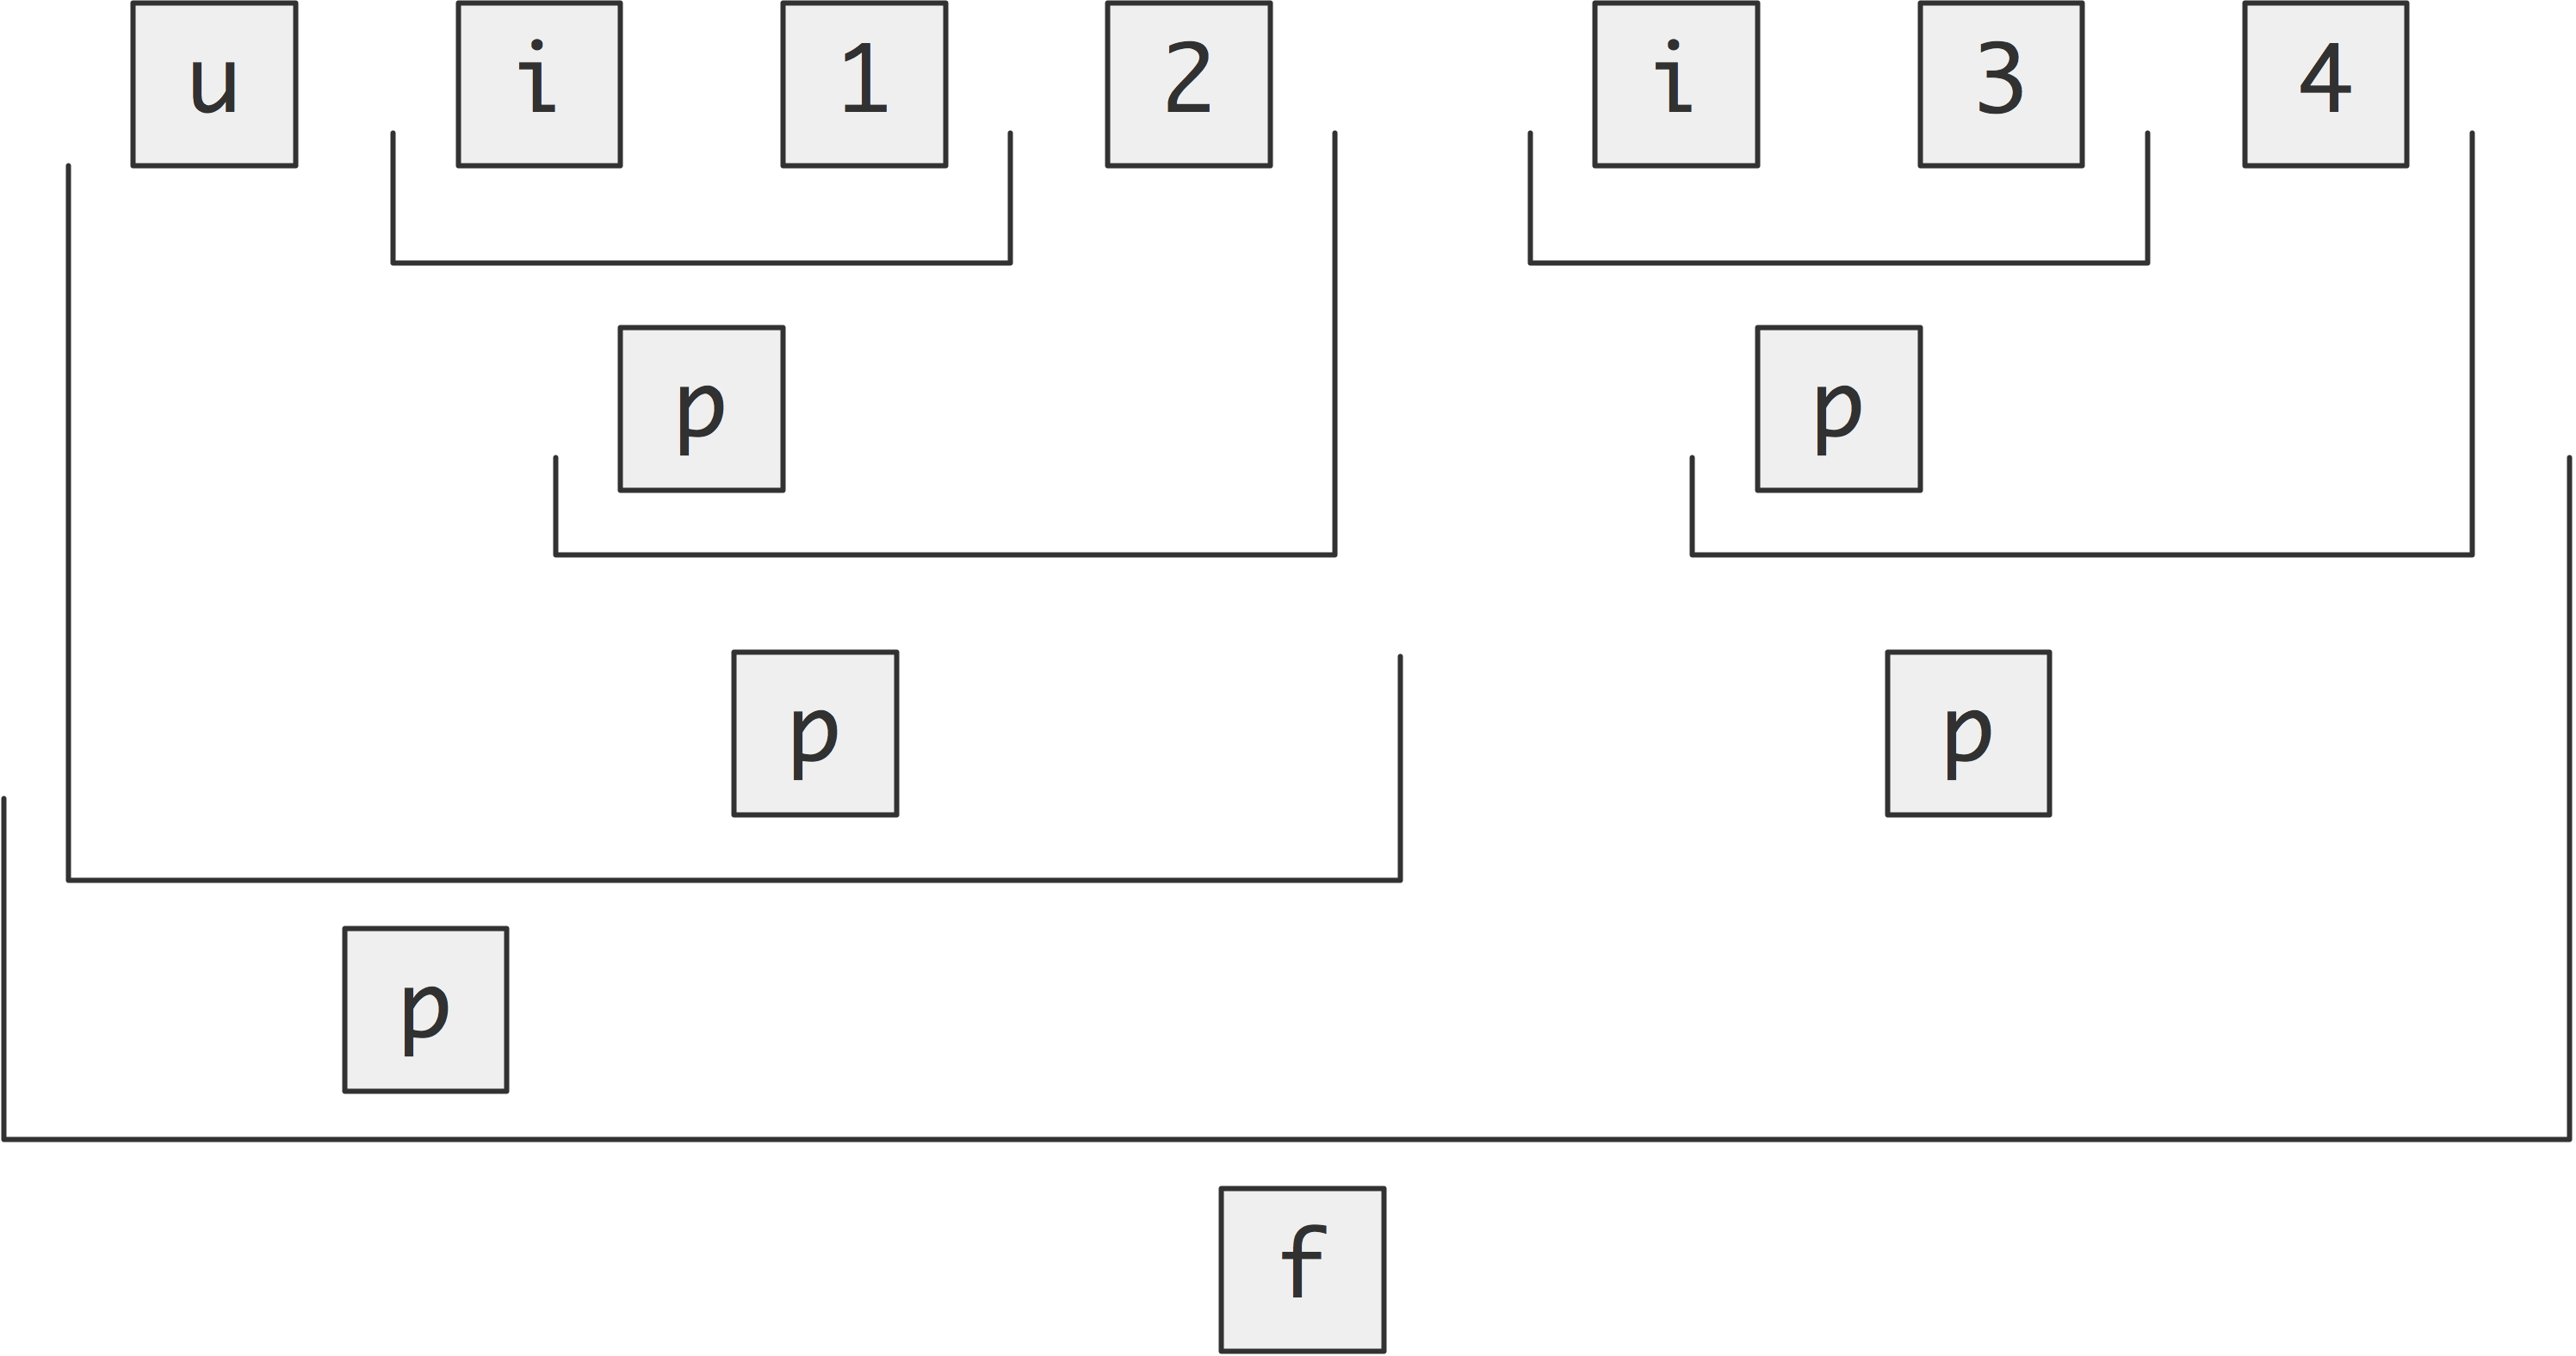
\includegraphics[scale=.1]{omp-reduct}
  \caption{Structure of a reduction of four items on two threads,
    where $u$ is the user-supplied initial value,
    and $i$~is the natural initial value for the reduction operator.}
  \label{fig:omp-reduct}
\end{figure}

OpenMP resolves the race condition on the reduction variable
by giving each thread a local copy of \lstinline{sum_of_squares},
summing into that, and adding the local copies together in the end.
This is illustrated in figure~\ref{fig:omp-reduct}.

%%packtsnippet end

\Level 1 {Five-point stencil}
%%packtsnippet d2d5pt
\label{sec:d2d-5pt}

The evaluation of the 5-point difference operator is perfectly parallel
in that there are no dependencies between the points of the output vector.
However, the loop is more complicated than the scaling operation above:
%
\cxxverbatimsnippet{d2d5ptseq}

While this operation is somewhat like a `transform' range operation,
the complexity of the right-hand-side indexing precludes using
an actual range algorithm.
Therefore, in later versions of this code we will range over
the indices, rather than the actual data.

%%packtsnippet end

\Level 0 {Parallelization strategies}

There are various ways we can parallelize our example application.

\Level 1 {OpenMP loop parallelism}

Above in section~\ref{sec:d2d-omp1d}
we already showed the simplest parallelization scheme:
we loop two-dimensionally over the index space,
and translate that through a \ac{CPP} macro
to one-dimensional indexing in a traditional container.
The loops are then parallelized by OpenMP.

In graphs to follow we indicate by~`\n{oned}'
the mode where we only parallelize the outer loop.
For instance, the norm calculation is:
%
\cxxverbatimsnippet{d2dnormomp}

We designate by `\n{clps}' this same code, but adding
\lstinline{collapse(2)} to each OpenMP loop nest.

\Level 1 {\texttt{mdspan} indexing}

While the scaling and the norm calculation can be expressed as range algorithms,
doing so for the five-point stencil update is trickier,
so we take a two-step approach:

  
\begin{enumerate}
\item We access data through an \lstinline{mdspan}, so that have multidimensional indexing;
  see figure~\ref{fig:data2d}

\begin{figure*}[h]
  \twosnippetswithcaptions{Class data:}{d2dspan0}{Accessor:}{d2dspan2}
  \caption{Use of \texttt{mdspan} for 2D data access}
  \label{fig:data2d}
\end{figure*}

\item We define the iteration space as a \indexc{cartesian_product} range view:

  \cxxverbatimsnippet{d2dinner}

\end{enumerate}
This allows us to write, cleanly and compactly:
%
\cxxverbatimsnippet{d2d5ptspan}
%
Unlike the OpenMP double loop, we now have a single loop
spanning the two-dimensional domain.
Also, note that this domain is the interior of a larger domain.

In graphs to follow we indicate this mode by~`\n{span}'.

In the tests below it will become apparent that the two-dimensional
iteration space is not without performance problems.
We tackle this by having a variant, `\n{iota}',
which splits the space orthogonally:
%
\cxxverbatimsnippet{d2dnormiota}

\Level 1 {DIY cartesian product}

The \lstinline{cartesian_product} view is quite general
so one could wonder about overhead.
We write a custom iterator over a contiguous domain.
It maintains internally \lstinline{i,j} coordinates
which are updated by the \lstinline{operator++}.
A~naive implementation uses integer division, so we also
make an optimized implementation without division or branching.
%
\twosnippetswithcaptions{Simple}{d2ddiyiter}{Optimized}{d2ediyiter}

\Level 1 {Kokkos and Sycl}

We also use the Kokkos and Sycl libraries in their `host' mode.
In graphs to follow we indicate these modes
by `\n{kokkos}' and `\n{sycl}' respectively.

\Level 2 {Sycl}

Sycl is an open standard that targets
heterogeneous parallelism through strict standard C++.
It has mechanisms for memory management between host CPU
and devices (both GPU and FPGA),
and for expressing common parallel algorithms.

The preferred mechanism for handling memory coherence is through buffers.
Host memory is wrapped in a buffer structure:
\cxxverbatimsnippet{syclbufcreate}

This memory can then transparently be accessed in a kernel,
whether run on host or device,
where coherence is ensured by the runtime.
This turns out to be as efficient as more explicit mechanisms.
%
\cxxverbatimsnippet{syclbufaccess}
%
Note that Sycl has a true two-dimensional indexing mode.

We see that the \lstinline{parallel_for} construct
resembles a C++ range algorithm: it combines
a range --~though of the index space, not the data space~--
and a lambda expression to be applied at each point.

Sycl is alone among the models studied here
in that it requires index shifting 
in order to range over the interior of the index space.

\Level 2 {Kokkos}

Kokkos is the execution layer of the Trilinos project.
It is, like Sycl, a data-parallel programming mode
that supports host and device execution with the same code.
Unlike Sycl there is no explicit queue; instead,
objects are explicitly associated with the host or device data space.

\cxxverbatimsnippet{kokkosbufcreate}

Like Sycl, there are explicit parallelism constructs.
These closely resemble C++ range algorithms,
specifying an explicit index space over which to iterate,
and the lambda expression to apply at each index.

\cxxverbatimsnippet{kokkosbufaccess}

\Level 0 {Timing comparison and discussion}

We perform different comparisons:
\begin{itemize}
\item different parallelization models on a given compiler and CPU;
\item different Intel processor generations, given a model and compiler;
\item different compilers, given a model and CPU.
\end{itemize}

\Level 1 {Comparing parallelization models}

Let's compare various implementation strategies.
Test given here are on an \indextermbus{Intel}{Sapphire Rapids}
dual socket node with 112 cores total.
We compare the Intel~2024 (figure~\ref{fig:diff2d-variants-intel})
and GCC~13 (figure~\ref{fig:diff2d-variants-gcc})
compilers.

\begin{figure*}[t]
  \pgfplotsset{table/col sep=comma}
  \begingroup %\begin{multicols}{2}
    \tikzsetnextfilename{diff2d-ratios-intel-spr}
    \begin{tikzpicture}
      \begin{semilogyaxis}[
          title=Execution time,
          ylabel=time (msec), xlabel=cores,
          width=.5\textwidth, height=.5\textwidth,
          legend entries={oned,clps,span,iota,diy2e,kokkos,sycl,},
          legend pos=north east,
        ]
        \addplot table[y=oned]{plots/spr-ratios-intel.csv};
        \addplot table[y=clps]{plots/spr-ratios-intel.csv};
        \addplot table[y=span]{plots/spr-ratios-intel.csv};
        \addplot table[y=iota]{plots/spr-ratios-intel.csv};
        \addplot table[y=diy2e]{plots/spr-ratios-intel.csv};
        \addplot table[y=kokkos]{plots/spr-ratios-intel.csv};
        \addplot table[y=sycl]{plots/spr-ratios-intel.csv};
      \end{semilogyaxis}
    \end{tikzpicture}
    %\columnbreak
    \tikzsetnextfilename{diff2d-ratios-intel-spr-sp}
    \begin{tikzpicture}
      \begin{axis}[
          title=Ratio to oned,
          ylabel=ratio, ymax=20, xlabel=cores,
          width=.5\textwidth, height=.5\textwidth,
          legend entries={oned,clps,span,iota,diy2e,kokkos,sycl,},
          legend pos=north west,
        ]
        \addplot table[y=oned]{plots/spr-ratios-intel-rat.csv};
        \addplot table[y=clps]{plots/spr-ratios-intel-rat.csv};
        \addplot table[y=span]{plots/spr-ratios-intel-rat.csv};
        \addplot table[y=iota]{plots/spr-ratios-intel-rat.csv};
        \addplot table[y=diy2e]{plots/spr-ratios-intel-rat.csv};
        \addplot table[y=kokkos]{plots/spr-ratios-intel-rat.csv};
        \addplot table[y=sycl]{plots/spr-ratios-intel-rat.csv};
      \end{axis}
    \end{tikzpicture}
  \endgroup %\end{multicols}
  \caption{Comparing implementation strategies, Intel 2024 compiler on a 112-core Sapphire Rapids node.}
  \label{fig:diff2d-variants-intel}
\end{figure*}

\begin{figure*}[t]
  \pgfplotsset{table/col sep=comma}
  \begingroup %\begin{multicols}{2}
    \tikzsetnextfilename{diff2d-ratios-gcc-spr}
    \begin{tikzpicture}
      \begin{semilogyaxis}[
          title=Execution time,
          ylabel=time (msec), xlabel=cores,
          width=.5\textwidth, height=.5\textwidth,
          legend entries={oned,clps,span,iota,kokkos,},
          legend pos=north east,
        ]
        \addplot table[y=oned]{plots/spr-ratios-gcc.csv};
        \addplot table[y=clps]{plots/spr-ratios-gcc.csv};
        \addplot table[y=span]{plots/spr-ratios-gcc.csv};
        \addplot table[y=iota]{plots/spr-ratios-gcc.csv};
        \addplot table[y=kokkos]{plots/spr-ratios-gcc.csv};
      \end{semilogyaxis}
    \end{tikzpicture}
    %\columnbreak
    \tikzsetnextfilename{diff2d-ratios-gcc-spr-sp}
    \begin{tikzpicture}
      \begin{axis}[
          title=Ratio to oned,
          ylabel=ratio, ymax=12, xlabel=cores,
          width=.5\textwidth, height=.5\textwidth,
          legend entries={oned,clps,span,iota,kokkos,},
          legend pos=north west,
        ]
        \addplot table[y=oned]{plots/spr-ratios-gcc-rat.csv};
        \addplot table[y=clps]{plots/spr-ratios-gcc-rat.csv};
        \addplot table[y=span]{plots/spr-ratios-gcc-rat.csv};
        \addplot table[y=iota]{plots/spr-ratios-gcc-rat.csv};
        \addplot table[y=kokkos]{plots/spr-ratios-gcc-rat.csv};
      \end{axis}
    \end{tikzpicture}
  \endgroup %\end{multicols}
  \caption{Comparing implementation strategies, Gcc 2024 compiler on a 112-core Sapphire Rapids node.}
  \label{fig:diff2d-variants-gcc}
\end{figure*}

We make the following observations.

\Level 2 {Intel compiler}

First of all, we see that the naive `\n{oned}' OpenMP implementation
is clearly the fastest.
All of the schemes that use two-dimensional iteration are slower.
An indication of the reason for this is outlined in section~\ref{sec:d2d-profile}:
much of the computing time actually goes into incrementing the
two-dimensional iterator.

If we accept a constant loss of efficiency for these schemes,
we see that most schemes even have a descending efficiency
with increasing core count.
The reason for this is not clear, especially since the
`\n{clps}' and `\n{diy}' implementations do not show this.

Interestingly, on low core counts the `\n{sycl}' and `\n{kokkos}'
implementations are relatively competitive.
They probably employ an efficient translation to an OpenMP backend,
but this makes their gradual loss of efficiency all the more puzzling.

\Level 2 {GNU compiler}

For the GNU compiler the differences between the various models
are much smaller.
Moreover, most models have constant efficiency, kokkos being the exception.

\Level 1 {Comparing processor generations}

%% RESULTS SHOWING COMPARISONS BETWEEN INTEL PROCESSOR GENERATIONS
%% REMOVED TO SATISFY PAGE LIMITS. THIS CAN BE REINSTATED FOR FINAL SUBMISSION.

%% \begin{comment}

\begin{figure*}[t]
  \pgfplotsset{table/col sep=comma}
  \hbox\bgroup %%\begin{multicols}{2}
    \tikzsetnextfilename{diff2d-procs}
    \begin{tikzpicture}
      \begin{semilogyaxis}[
          title=Runtime,
          ylabel=time (msec), xlabel=cores,
          width=.55\textwidth, height=.5\textwidth,
          legend entries={skx,clx,icx,spr,grx},
        ]
        \addplot table[y=skx]{plots/gcc-oned-skx-26000.csv};
        \addplot table[y=clx]{plots/gcc-oned-clx-26000.csv};
        \addplot table[y=icx]{plots/gcc-oned-icx-26000.csv};
        \addplot table[y=spr]{plots/gcc-oned-spr-26000.csv};
        \addplot table[y=grx]{plots/gcc-oned-grx-26000.csv};
      \end{semilogyaxis}
    \end{tikzpicture}
    %% \columnbreak
    \tikzsetnextfilename{diff2d-procs-bw}
    \begin{tikzpicture}
      \begin{axis}[
          title=Bandwidth,
          ylabel=BW (Gb/s), xlabel=cores,
          width=.55\textwidth, height=.5\textwidth,
          legend entries={skx,clx,icx,spr,grx},
          legend pos=north west,
        ]
        \addplot table[y=skx]{plots/gcc-oned-skx-26000-bw.csv};
        \addplot table[y=clx]{plots/gcc-oned-clx-26000-bw.csv};
        \addplot table[y=icx]{plots/gcc-oned-icx-26000-bw.csv};
        \addplot table[y=spr]{plots/gcc-oned-spr-26000-bw.csv};
        \addplot table[y=grx]{plots/gcc-oned-grx-26000-bw.csv};
      \end{axis}
    \end{tikzpicture}
  \egroup %%\end{multicols}
  \caption{Generations of Intel processors (OpenMP). Time (left) and speedup (right) as function of core count.}
  \label{fig:diff2d-procs}
\end{figure*}

In figure~\ref{fig:diff2d-procs} we compare the following generations of Intel processors:
\begin{itemize}
\item \indextermbus{Intel}{Sky Lake} in the \indextermbus{TACC}{Stampede2} cluster,
  in a two-socket configuration with a total of 48 cores;
\item \indextermbus{Intel}{Cascade Lake} in the \indextermbus{TACC}{Frontera} cluster,
  in a two-socket configuration with a total of 56 cores;
\item \indextermbus{Intel}{Ice Lake} in the \indextermbus{TACC}{Stampede3} cluster,
  in a two-socket configuration with a total of 80 cores;
\item \indextermbus{Intel}{Sapphire Rapids} in the \indextermbus{TACC}{Stampede3} cluster,
  in a two-socket configuration with a total of 112 cores;
\item \indextermbus{Intel}{Granite Rapids} in the \indextermbus{TACC}{Stampede3} cluster,
  in a two-socket configuration with a total of 240 cores;
\end{itemize}

\Level 2 {Runtime}

In the left graph we see that the runtimes are roughly equal for low core counts;
the main difference is that Sky Lake and Cascade Lake reach their maximum performance
well short of the total core count, while Ice Lake does not show this behavior.
The Ice Lake and later generations keep scaling with increasing core count,
the both Rapids generations even almost linearly.

\Level 2 {Bandwidth}

Our bandwidth measure is not observed directly, but
rather derived by considering the amount of data loads
in the algorithm:
\begin{itemize}
\item The five-point stencil application loads 5~elements from the input,
  loads the output vector, and writes it; this would come to 7~data accesses per
  $i,j$ point calculation.
\item However, subsequent points from each $i$ or $i-1$ or $i+1$ line
  come from the same cacheline, so effectively we 3~accesses from the input vector,
  for 5~total.
\item Added to this, lines easily fit in L2 cache, so after the line for one
  $i+1$~value has been loaded, it will be used as the $i$ line
  in the next iteration, and the $i-1$ line in the iteration thereafter.
  Thus, we really have only 1~DRAM access for the input vector per $i,j$ point calculation,
  for a total of 3~access.
\item Finally, the Ice Lake processor can, in certain circumstances,
  convert the calculation to a `streaming store', so the load of the output vector
  doesn't need to be counted.
\end{itemize}

The right graph of figure~\ref{fig:diff2d-procs} shows a \emph{a~posteriori}
measure for attained bandwidth.

%% \end{comment}

We see that the Sky Lake and Cascade Lake processors bear out the
old truism that the total bandwidth is less than 
each core's individual bandwidth summed over the cores.

However, newer processor generations scale further, and
for the Sapphire Rapids and Granite Rapids even fairly linear.
The SPR node has Intel's `High Bandwidth Memory',
given a much higher absolute number.

\Level 1 {Comparing compilers}

\begin{figure*}[t]
  \pgfplotsset{table/col sep=comma}
  \begingroup %\begin{multicols}{2}
    \tikzsetnextfilename{oned-ratios-spr-sp}
    \begin{tikzpicture}
      \begin{semilogyaxis}[
          title=Ratio GCC to Intel on oned,
          xlabel=cores,
          ylabel=ratio, ymin=.1, ymax=10, 
          ytickten={-1,-.5,0,0.5,1},
          yticklabels={1/10,1/3,1,3,10},
          width=.5\textwidth, height=.5\textwidth,
          legend entries={intel,gnu,},
          legend pos=north west,
        ]
        \addplot table[y=intel]{plots/oned-ratios-iccgcc-rat.csv};
        \addplot table[y=gnu]{plots/oned-ratios-iccgcc-rat.csv};
      \end{semilogyaxis}
    \end{tikzpicture}
    \tikzsetnextfilename{clps-ratios-spr-sp}
    \begin{tikzpicture}
      \begin{semilogyaxis}[
          title=Ratio GCC to Intel on clps,
          xlabel=cores,
          ylabel=ratio, ymin=.1, ymax=10, 
          ytickten={-1,-.5,0,0.5,1},
          yticklabels={1/10,1/3,1,3,10},
          width=.5\textwidth, height=.5\textwidth,
          legend entries={intel,gnu,},
          legend pos=north west,
        ]
        \addplot table[y=intel]{plots/clps-ratios-iccgcc-rat.csv};
        \addplot table[y=gnu]{plots/clps-ratios-iccgcc-rat.csv};
      \end{semilogyaxis}
    \end{tikzpicture}
  \endgroup %\end{multicols}
  \caption{Comparing Intel to GCC on `oned' (left) and `clps' (right) scheme}
  \label{fig:compiler-compare-oned}
\end{figure*}

\begin{figure*}[t]
  \pgfplotsset{table/col sep=comma}
  \begingroup %\begin{multicols}{2}
    \tikzsetnextfilename{span-ratios-spr-sp}
    \begin{tikzpicture}
      \begin{semilogyaxis}[
          title=Ratio GCC to Intel on span,
          xlabel=cores,
          ylabel=ratio, ymin=.1, ymax=10, 
          ytickten={-1,-.5,0,0.5,1},
          yticklabels={1/10,1/3,1,3,10},
          width=.5\textwidth, height=.5\textwidth,
          legend entries={intel,gnu,},
          legend pos=north west,
        ]
        \addplot table[y=intel]{plots/span-ratios-iccgcc-rat.csv};
        \addplot table[y=gnu]{plots/span-ratios-iccgcc-rat.csv};
      \end{semilogyaxis}
    \end{tikzpicture}
    \tikzsetnextfilename{kokkos-ratios-spr-sp}
    \begin{tikzpicture}
      \begin{semilogyaxis}[
          title=Ratio GCC to Intel on kokkos,
          xlabel=cores,
          ylabel=ratio, ymin=.1, ymax=10, 
          ytickten={-1,-.5,0,0.5,1},
          yticklabels={1/10,1/3,1,3,10},
          width=.5\textwidth, height=.5\textwidth,
          legend entries={intel,gnu,},
          legend pos=north west,
        ]
        \addplot table[y=intel]{plots/kokkos-ratios-iccgcc-rat.csv};
        \addplot table[y=gnu]{plots/kokkos-ratios-iccgcc-rat.csv};
      \end{semilogyaxis}
    \end{tikzpicture}
  \endgroup %\end{multicols}
  \caption{Comparing Intel to GCC on `span' (left) and `kokkos' (right) scheme}
  \label{fig:compiler-compare-span}
\end{figure*}

Figures \ref{fig:compiler-compare-oned} and \ref{fig:compiler-compare-span}
show a comparison between the Intel 2024 and GCC 13 compilers.
While sometimes Intel has a slight edge over GCC, it sometimes
performs considerably worse.
Inspection of the generated code would be needed to determine the cause of this.

\Level 1 {Analysis}
\label{sec:d2d-profile}

One immediate conclusion from the above tests is that it's
hard to beat the simple-minded OpenMP implementation
with only the outer loop parallelized,
although differences are less pronounced for the Gnu compiler
than the Intel one.

Doing profiling gives us a clue.
Here is the output of running the \indexc{mdspan}~/ \indexc{cartesian_product}
version (Intel 24 compiler):
\begin{lstlisting}[language=verbatim]
%% make run_perf VARIANTS=span NSIZE=10000 ECHO=1  

    55.60%  [.] std::ranges::cartesian_product_view<std::ranges::iota_view<long, long>, std::ranges::iota_view<long, long> >::_Iterator<true>::operator+=
    18.73%  [.] __divti3
    11.33%  [.] linalg::bordered_array_span<float>::central_difference_from
     5.37%  [.] linalg::bordered_array_span<float>::scale_interior
     5.01%  [.] linalg::bordered_array_span<float>::l2norm
     2.69%  [.] __divti3@plt
\end{lstlisting}
We see that more than half of the time goes into index calculations,
and in particular integer division.

\begin{comment}
  This makes send if we consider our `diy' implementation:
  \cxxverbatimsnippet{d2ddiyiter}
  Unfortunately it's not the plus-plus operator but the plus-and-is,
  which is the bottlenect.
  For the former we can come up with trickery to lose the divisions:
  \cxxverbatimsnippet{d2ddiziter}
  for the latter that's much harder.
  (Note that the tricked code has no conditionals that could give branch mispredictions!)

  Unfortunately, \indexterm{perf} does not help us much here:
  \begin{lstlisting}[language=verbatim]
    35.25%  [.] linalg::bordered_array_diy2e<float>::l2norm
    31.39%  [.] linalg::bordered_array_diy2e<float>::central_difference_from
    30.46%  [.] linalg::bordered_array_diy2e<float>::scale_interior
    2.29%  [.] linalg::bordered_array_diy2e<float>::set
  \end{lstlisting}
  We get no timings for the embedded iterator.
  Note the counterintuitive result that the norm computation takes more time than the
  central difference,
  despite the latter having more operations
  and more complicated memory access.
\end{comment}

VTune profiling tells us something similar
(with some post-processing):
\begin{lstlisting}[language=verbatim]
std::ranges::cartesian_product_view<std::ranges::iota_view<long, long>, std::ranges::iota_view<long, long>>::_Iterator<(bool)1>::operator+= 44.15438
 linalg::bordered_array_span<float>::central_difference_from 12.71539
                  linalg::bordered_array_span<float>::l2norm 10.88307
          linalg::bordered_array_span<float>::scale_interior 9.63805
                                               func@0x404390 8.09852
                                                    __divti3 8.09808
                                                __udivmodti4 4.61700
     linalg::bordered_array_span<float>::bordered_array_span 0.87979
                     linalg::bordered_array_span<float>::set 0.87910
                              __kmp_get_global_thread_id_reg 0.00000
                     cfree 0.03664
\end{lstlisting}

\Level 0 {Conclusion}

We have implemented a stencil code, which stands for many scientific applications,
using various modern C++ mechanisms.
The tentative conclusion is that the modern mechanisms may be simpler to code,
but this elegance comes with a certain perforance penalty,
more so for the Intel compiler than the GCC compiler.

\endinput

%%%%
%%%% old stuff
%%%%

First of all we remark that ranging over data:
\begin{multicols}{2}
\begin{lstlisting}
#pragma omp parallel for 
for ( int i=0; i<x.size(); ++i )
  x[i] = f(i);
\end{lstlisting}
\columnbreak
\begin{lstlisting}
#pragma omp parallel for 
for ( auto& [i,e] : 
        x | rv::enumerate )
  e = f(i);
\end{lstlisting}
\end{multicols}
comes with zero performance penalty.

There are also `execution policies' but at the high core counts common in HPC,
these can be dramatically worse than using OpenMP.

%%%%
%%%% old tables
%%%%

\begin{figure}[t]
  \pgfplotsset{table/col sep=comma}
  \begin{multicols}{2}
    \tikzsetnextfilename{diff2d-strategies-lin}
    \begin{tikzpicture}
      \begin{semilogyaxis}[
          title=Scaling of diff2d application various implementations,
          ylabel=msec, xlabel=cores,
          width=.5\textwidth, height=.5\textwidth,
          legend entries={omp,clps,rng,sycl,},
        ]
        \addplot table[y=clps]{plots/diff2d-scaling-clps-spr-intel-25000.cvs};
        \addplot table[y=omp]{plots/diff2d-scaling-omp-frontera25000.csv};
        \addplot table[y=clps]{plots/diff2d-scaling-omp-frontera25000.csv};
        \addplot table[y=rng]{plots/diff2d-scaling-omp-frontera25000.csv};
        \addplot table[y=span]{plots/diff2d-scaling-omp-frontera25000.csv};
      \end{semilogyaxis}
    \end{tikzpicture}
   \columnbreak
   \tikzsetnextfilename{diff2d-strategies-loglog}
    \begin{tikzpicture}
      \begin{loglogaxis}[
          title=log-log display of same data,
          ylabel=msec, xlabel=cores,
          width=.5\textwidth, height=.5\textwidth,
          legend entries={omp,clps,rng,span,},
        ]
        \addplot table[y=omp]{plots/diff2d-scaling-omp-frontera25000.csv};
        \addplot table[y=clps]{plots/diff2d-scaling-omp-frontera25000.csv};
        \addplot table[y=rng]{plots/diff2d-scaling-omp-frontera25000.csv};
        \addplot table[y=span]{plots/diff2d-scaling-omp-frontera25000.csv};
      \end{loglogaxis}
    \end{tikzpicture}
  \end{multicols}
  %% \addplot table[y=linear]{plots/fivepoint-scaling-frontera6000.csv};
  \caption{Different approaches to OpenMP parallelization of a five-point Laplace loop.}
  \label{fig:diff2d-strategies}
\end{figure}

\begin{figure}[t]
  \pgfplotsset{table/col sep=comma}
  \begin{multicols}{2}
    \tikzsetnextfilename{diff2d-variants-gcc}
    \begin{tikzpicture}
      \begin{axis}[
          title=Speedup with Intel compiler,
          ylabel=speedup, ymax=100, xlabel=cores,
          width=.5\textwidth, height=.5\textwidth,
          legend entries={seq,kokkos,oned,span,},
          legend pos=north west,
        ]
        \addplot table[y=seq]{plots/diff2d-scaling-seq-clx-gcc-40000-sp.csv};
        \addplot table[y=kokkos]{plots/diff2d-scaling-seq-clx-gcc-40000-sp.csv};
        \addplot table[y=oned]{plots/diff2d-scaling-seq-clx-gcc-40000-sp.csv};
        \addplot table[y=span]{plots/diff2d-scaling-seq-clx-gcc-40000-sp.csv};
      \end{axis}
    \end{tikzpicture}
    \columnbreak
    \tikzsetnextfilename{diff2d-variants-intel}
    \begin{tikzpicture}
      \begin{axis}[
          title=Speedup with GCC compiler,
          ylabel=speedup, ymax=100, xlabel=cores,
          width=.5\textwidth, height=.5\textwidth,
          legend entries={seq,kokkos,oned,span,},
          legend pos=north west,
        ]
        \addplot table[y=seq]{plots/diff2d-scaling-seq-clx-intel-40000-sp.csv};
        \addplot table[y=kokkos]{plots/diff2d-scaling-seq-clx-intel-40000-sp.csv};
        \addplot table[y=oned]{plots/diff2d-scaling-seq-clx-intel-40000-sp.csv};
        \addplot table[y=span]{plots/diff2d-scaling-seq-clx-intel-40000-sp.csv};
      \end{axis}
    \end{tikzpicture}
  \end{multicols}
  \caption{Various implementation strategies; speedup as function of core count}
  \label{fig:diff2d-variants}
\end{figure}

